\chapter{Knihovna pro práci s regulárními výrazy}\label{sec:Implementation1}

Jako prvotní myšlenka před tvorbou samotné vizualizace, jsem měl úvahu o použití knihovny, 
která by mi umožňovala zpracovávat regulární výrazy.
Sice implementace regulárních výrazů se nachází v samotné specifikaci JavaScriptu,
ale ta mi neumožňuje získat informaci o samotném vyhledávání.
Po prozkoumání, zda-li existují řešení, která by vyhovovala této práci, 
jsem uznal za vhodné, vytvořit vlastní implementaci v podobě této knihovny.
Nenaleznul jsem totiž řešení, které by bylo dostatečně flexibilní a 
zároveň lehce integrovatelné do programovacího jazyku TypeScript.
Sice vlastní implementace je pracná, ale jelikož chci mít co nejvyšší kontrolu nad výslednou strukturou, 
tak je toto řešení pro tuto aplikaci asi nejvhodnější. 

V této části práce se pokusím vysvětlit, jak je naimplementována tato knihovna \ref{sec:Imp1LayoutReal}, 
jaké problémy se ukázali při vývoji a její výhody a nevýhody. % TODO: references

\section{Rozvržení}\label{sec:Imp1LayoutReal}

Vstupní třídou, pro tuto knihovnu je \textbf{Regexer}. 
Slouží jako spojující a zároveň obsluhující třída. 
Zároveň poskytuje rozhraní této knihovny.
Dále si drží důležité informace, které souvisí s aktuálním regulárním výrazem.
\textbf{RegexMatch} je třída, která reprezentuje jeden výsledek vyhledávání zadaným výrazem.
Její data jsou soukromá, ale umožňuje je procházet pomocí svých metod.
Jedna instance teto třídy, je ekvivalentní jednomu vyhledání v textu.
Data této třídy jsou generována třídou \textbf{MatchBuilder}.
Instance této třídy existuje jen ve chvíli, kdy probíhá vyhledávání v zadaném řetězci.
Poskytuje rozhraní, které umožňuje přidávat stavy, s tím že může tato data upravovat, dle své potřeby.
Tento objekt je pak držený v tříde \textbf{MatcherInternal}, 
která má za ůkol, průchod zadaným řetězcem, pro konkrétní výraz.
Tato třída, je izolována a není dostupná z vnější, jak její název internal, v překladu vnitřní napovídá.
Obsahuje hlavní logickou část průchodu nedeterministickým automatem.
Naopak třídou, která poskytuje vyditelné rozhraní a volá metody třídy MatcherInternal je \textbf{Matcher}.
Její rozhraní je poskytováno třídě Regexer.
Pro parsování textové reprezentace regulárního výrazu na strukturu, slouží rozhraní \textbf{RegexParser}.
Vzniká vždy po překladu bezkontextové gramatiky.
Jako poslední struktura, která stojí za zmínku, je \textbf{Stack}.
Stack nebo-li zásobník, je velmi důležitou součástí vyhledávání.
Zásobník je totiž struktura, která mi dovoluje se zbavit rekurzivního volání funkce.
Rekurze obecně vede k pomalejšímu chodu programu a nelze ji jednoduše pozastavit v jakémkoliv čase.
Také může jednoduše při složitějším zpracování dojít k přetečení zásobníku, který je často limitován aby nedošlo k nekonečnému rekurzivnímu volání.
Sice rozhraní pole v JS je připraveno na funkcionalitu zásobníku, ale nezaručuje programátorovi daná pravidla pro zásobník. 
Z tohoto důvodu jsem zvolil jednoduchou implementaci zásobníku, která omezuje manipulaci s základním polem, na operace určené pro zásobník.

Vztahy mezi jednotlivými třídami, lze vidět na obrázku \ref{fig:ARCH_RGXR}. 
Myslím si že je vhodné poukázat na obalující blok \textbf{MatchingWorker}.
Jedná se o vstupní soubor vedlejšího vlákna, který slouží pro asynchroní komunikaci s hlavním vláknem.


% Je-li vytvořena instance této třídy, je potřeba parsnout zadaný regulární výraz, pomocí metody \textbf{parse}.
% Regexer, jako řídící třída zavolá RegexParser, který dokáže zpracovat textovou podobu regulárního výrazu na strukturu AST a NKA.
% TODO ^ update, change location probbably

\begin{figure}[!h]
	\centering
	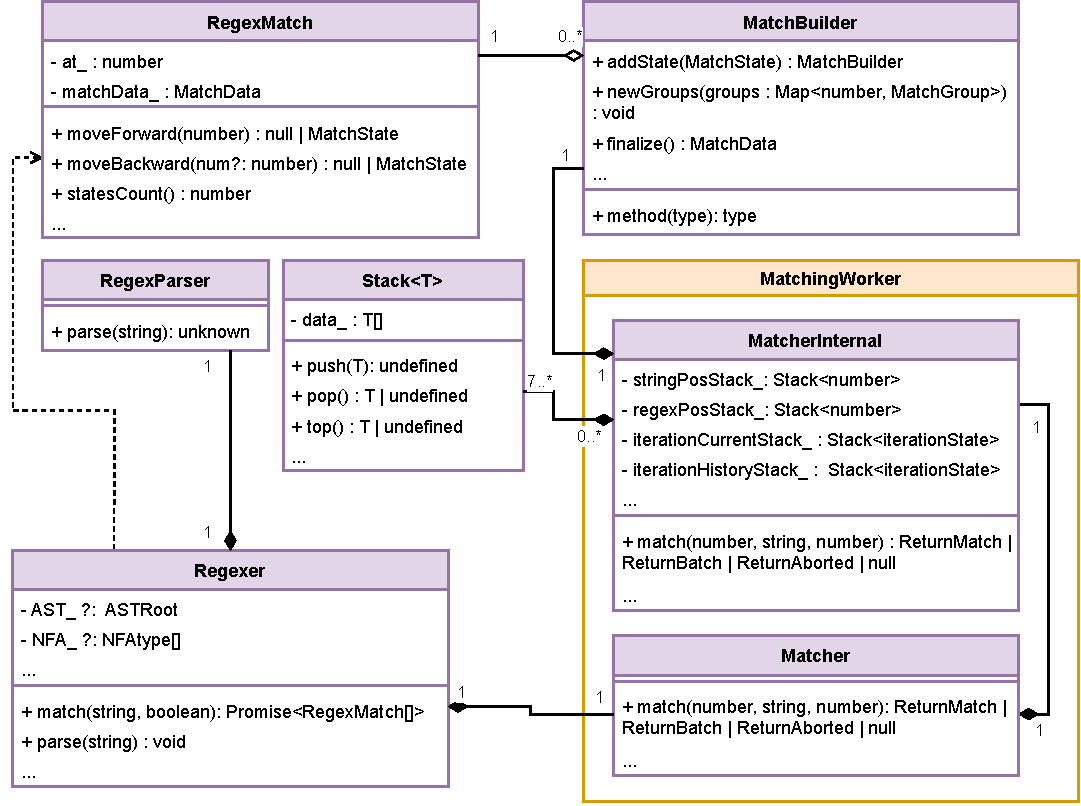
\includegraphics[width=0.9\textwidth]{Figures/UML_RGXR.pdf}
	\caption{Třídní diagram části knihovny pro práci s regulárními výrazy}
	\label{fig:ARCH_RGXR}
\end{figure}

\section{Parsování regulárních výrazů}

\subsection*{Parser}

Jak již bylo zmíněno, pro parsování regulárních výrazu jsem použil bezkontextovou gramatiku Peggy.
Jedná se o pokračování projektu pegjs, ale ten se již dlouho nevyvíjí. 
Jelikož tato knihovna je stále aktualizována a má velkou podporu vývojářů, tak jsem zvolil její využití pro tuto práci.

V ukázce \ref{code:grammar1} se nachází vstupní neterminál bezkontextové gramatiky. 
Ten obsahuje výběr mezi dvěma začátky.
Výběr je pak dostupný pod názvem \textit{type}, podle toho který se zvolí.
Před dokončením pravidla a vracením dat, se zde může nacházet jejich modifikace.
%TODO: move somewhere \/
%Tato modifikace je uzavřená ve složených závorkách \{\} a data po změně jsou vrácena pomocí return.
Modifikace v rámci pravidla začátku, probíhá zavoláním instance vlastní třídy \textbf{ParserHandler}, která je součástí gramatiky.
Třída má za ůkol zpracovávat příchozí data do struktury, která je ukázaná na obrázku \ref{fig:JSONex}.

\begin{code}[!ht]
	\begin{minted}{peg}
start 
	= 
	type:(moded_start / general_start)
	{
		const data = { modifiers: type?.modifiers };
		return handler.handle(data, type?.elements, States.ROOT);
	}
	\end{minted}
	\caption{Počáteční neterminál}
	\label{code:grammar1}
\end{code}

Existuje několik různých vzorů regulárních výrazů.
Každý ze vzorů má pravidla, podle toho s jakými vzory je lze kombinovat.
Ukázka kódu \ref{code:grammar2}, obsahuje všechny možné výběry pravidel, které jsem naimplementoval pro parsování výrazů.
Například možnosti pro iteraci, ve zmíněném kódu \textit{to\_iterate}, obsahují pouze následující vzory, které mohou být opakovány.

\begin{itemize}
	\item Speciální znaky (\textit{escaped\_special}) -- $\textbackslash s$, $\textbackslash d$
	\item Základní znaky (\textit{primitive}) -- $a$, $b$, $0$
	\item Výběr jakéhokoliv znaku (\textit{any\_character}) -- $.$
	\item Skupina (\textit{group}) -- $()$
	\item List znaků (\textit{list}) -- $[a-z]$
\end{itemize}

V mnoha případech záleží na pořadí výběru z dostupných vzorů, proto je potřeba určit, které možnosti upřednostit.
Abych vysvětlil, proč je pořadí důležité vybral jsem si příklad \textbf{iterace} (iteration) a \textbf{výběru} (option).
Výběr má vyšší přednost, jelikož může mít za potomka iteraci.
Kdyby se iterace nacházela před výběrem, tak by došlo k tomu že by nebyla součástí výběru, pokud by byla jako první možnost. 
Nebo-li byla by dříve zpracována, než-li samotný výběr.
Příkladem může být výraz $a*|b*$, při kterém by se první zpracovala iterace $a*$.
Výsledkem výběru by byly 2 možnosti $\epsilon$ nebo $b*$, což je sice sám o sobě správný tvar, ale ve zvoleném výrazu \textbf{musí} být výběr $a*$ nebo $b*$.

\begin{code}[!ht]
	\begin{minted}{peg}
general
	= list / escaped_special / primitive / any_character / lookaround / group / EOS / SOS

any_element 
	= option / iteration / optional / general

to_iterate
	= escaped_special / primitive / any_character / group / list

to_option
	= iteration / optional / general

to_optional 
	= escaped_special / primitive / any_character / group / list

to_list
	= escaped_special / range_ascii / hexadecimal_ascii / [^\]\\] / is_escaped
	\end{minted}
	\caption{Výběry členů, pro všechny vzory regulárních výrazů, podle náležitých pravidel}
	\label{code:grammar2}
\end{code}

\subsection*{Struktura zpracovaného regulárního výrazu}

Pro zpracovaný regulární výraz, jsem zvolil strukturu, která obsahuje \textbf{nedeterministický konečný automat}, zároveň s \textbf{abstraktním syntaktickým stromem} (AST), 
ten pak slouží k dohledání informací o původním regulárním výrazu. 
Výsledná struktura je datového typu, JSON (JavaScript Object Notation).
JSON strukturu je možno vidět na obrázku \ref{fig:JSONex}.
NKA je ve formě \textbf{přesunové tabulky (transition table)}. 
Ta má tvar pole, kde každá položka obsahuje informaci o konktrétním stavu a přesunech na další stavy.
Stav se pak identifikuje na základě indexu v poli. 
Přesuny jsou pak implementovány tak, že každý stav si uchovává všechny přesuny, které vedou z daného stavu do stavu jiného.
Každý přesun pak má informaci, o jaký znak přesunu se jedná a na jaký index (stav) v poli odkazuje. 

Na obrázku \ref{fig:JSONex} lze vidět základní JSON struktura, která obsahuje dvě vstupní hodnoty AST a NFA.
Klíč NFA odkazuje na pole stavů přesunové tabulky. 
AST má odkaz na kořen, který signalizuje začátek regulárního výrazu.
Je zde patrné, že každý stav má odkaz, na příslušící prvek v AST. 
AST element drží různé informace, např. pozice v původním řetězci (start a end), 
potomci daného stavu, nebo typ elementu. 
Ne každý stav musí mít potomky, ale například skupina potomy má.

\begin{figure}[!h]
	\centering
	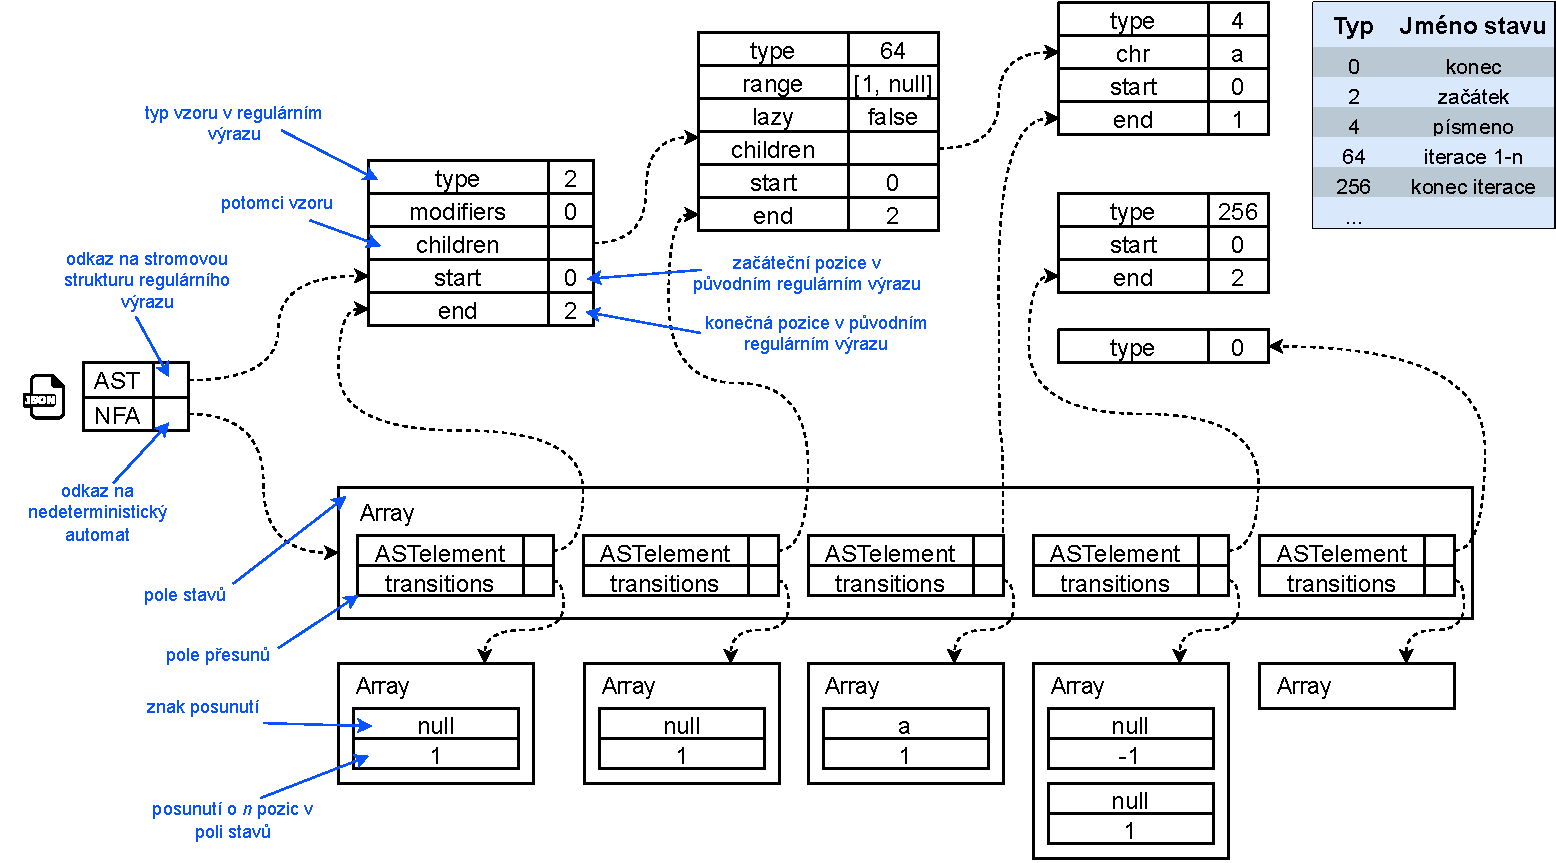
\includegraphics[width=1\textwidth]{Figures/BP-JSON.pdf}
	\caption{Příklad výsledné JSON struktury regulárního výrazu a+}
	\label{fig:JSONex}
\end{figure}

\section{Vyhledání pomocí regulárního výrazu}

%TODO: popsat výslednou strukturu
Vyhledání je hlavní částí této knihovny, jedná se o procházení regulárním výrazem a hledaným řetězcem.
Výsledkem je struktura JSON dat, která obsahuje informace o zpracovaném vyhledávání.
V této části textu popisuju, jak jsem naimplementoval vyhledávání, důležité koncepce a výslednou strukturu.

\subsection*{Odstranění rekurze}

Rekurze je sice důležitá v programování a dokáže usnadnit mnoho problémů, ale existují situace, kdy se vyplatí zbavit rekurze.
V první řadě, bych rád vysvětlil, proč se vůbec rekurzivní řešení hodí, pro vyhodnocování regulárních výrazů.
Jak jsem již zmínil, tak v regulárním výrazu může dojít k backtrackingu.
Nastane ve chvíli, kdy není možné z daného stavu v NKA, přejít na jiný stav.
V tuto chvíli, dojde k vrácení se v NKA do předchozích stavů a následnému vyhledávání další možné cesty.
Nejjednoduší řešení tohoto případu, je použití rekurze.
Pro představu, přechod značí rekurzivní volání funkce a pokud není možné přejít do dalšího stavu, tak se vrací do předozího volání funkce.

Rekurzi lze odstranit pomocí vlastních zásobníků, nebo-li program si uloží, jen potřebné informace a ve chvíli kdy dojde k vrácení se, tak vrch zásobníků se odstraní.
Důležité tedy je, správně řídit správu zásobníků, což může být komplikované.

Úryvek zdrojového kódu \ref{code:matching1}, obsahuje základní vkládání do zásobníku, konkrétně osahující stavy NKA a index aktuálního přesunu.
Pokud se stav již nachází na vrchu zásobníku, tak je pouze navýšen index přesunu.

% code pushing new state to stack
\begin{code}[!ht]
	\begin{minted}{typescript}
const nfaState = NFA[<number>this.regexPosStack_.top()] as NFAtype;
let topState = this.statesStack_.top();
if(topState?.state !== nfaState)
	this.statesStack_.push({transition: 0, state: nfaState});
else
	topState.transition++;
	\end{minted}
	\caption{Uložení stavu do zásobníku}
	\label{code:matching1}
\end{code}

Příklad kódu \ref{code:matching2}, souvisí s předchozí ukázkou. 
Jestli nastane situace, kdy neexistuje žádný další přesun z aktuálního stavu, je vyvolán backtracking.
Metoda \textit{handleBacktracking} se stará o správu backtrackingu.
Převážně se stará o odebírání vrchů zásobníků, jako je již zmíněný zásobník stavů.
Pokud není vrácená hodnota \textbf{null}, znamená to ukončení nebo pozastavení vyhledání.
K ukončení dojde, pokud je zásobník stavů vyprázněný a pozice v hledaném řetězci je na konci.

% code poping state from stack
\begin{code}[!ht]
	\begin{minted}{typescript}
const transitions = (nfaState as NFAState).transitions;
if(transitions.length <= <number>this.statesStack_.top()?.transition)
{
	const returned = this.handleBacktracking();
	if(returned !== null) return returned;
	continue;
}
	\end{minted}
	\caption{Vyvolání backtrackingu, pokud neexistují další přechody ze součastného stavu}
	\label{code:matching2}
\end{code}

\newpage

\subsection*{Počítání iterací a prevence nekonečných cyklů}

\begin{figure}[!h]
	\centering
	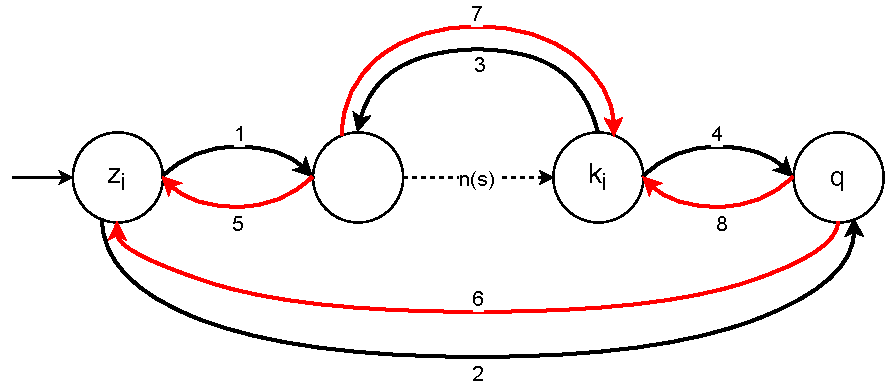
\includegraphics[width=1\textwidth]{Figures/IterationCount.pdf}
	\caption{NKA pro popis počítání iterací a prevenci nekonečných cyklů}
	\label{fig:ITERCNT}
\end{figure}

V seznamu pravidel, $I_i$ značí identifikátor iterace, $i$ je počet dokončených opakování iterace a $P_s$ je aktuální pozice v hledaném řetězci.
$I_{arr}$ obsahuje informace v poli o jedné iteraci [$I_i$, $i$, $P_s$].

Algoritmus pracuje se dvěma zásobníky, určenými pro držení informací o iteracích. 
První uchovává aktuálně nedokončené, resp. probíhající iterace. 
Pro popis jej označuji $Z_s$ (\textbf{zásobník současných iterací}).
Druhý značím jako $Z_h$ (\textbf{zásobník historie}), ten slouží pro iterace, které byly již dokončené.
Historie je důležitá pro backtracking.

\begin{enumerate}[label=\arabic* --]
	\item Vlož do $Z_s$ $\longleftarrow$ [$I_i$, 0, $P_s$]
	\item Vlož do $Z_h$ $\longleftarrow$ [$I_i$, 0, $P_s$]
	\item Vrchol $Z_s$, $I_{arr}$[1] + 1
	\item Vlož do $Z_h$ $\longleftarrow$ Odeber ze $Z_s$, $I_{arr}$[1] + 1
	\item Odeber ze $Z_s$
	\item Odeber ze $Z_h$
	\item Vrchol $Z_s$, $I_{arr}$[1] - 1
	\item Vlož do $Z_s$ $\longleftarrow$ Odeber ze $Z_h$, $I_{arr}$[1] - 1
\end{enumerate}

Na obrázku \ref{fig:ITERCNT} lze vidět nedeterministický automat. 
Jedná se o obecnou reprezentaci iterace, kde $z_i$ reprezentuje začátek iterace, $k_i$ konec iterace a $q$ značí první stav za iterací.
Mezi $z_i$ a $k_i$ se nachází množina stavů $n(s)$.
Červené šipky signalizují backtracking a černé značí klasický přechod mezi stavy.

Jelikož existují iterace v rozmezí, například od 3 do 6, tak je potřeba znát informaci, v kolikátém opakování se právě konkrétní iterace nachází.
Pro tento problém jsem zvolil 8 pravidel, které popisují řešení osmi různých přesunů mezi stavy.
Tato pravidla jsou rozepsána pod obrázkem \ref{fig:ITERCNT}, indexy pravidel korespondují s indexy v obrázku.
Rád bych poukázal, že při backtrackingu se vždy zásobníky vrací, do původních stavů. 
To znamená, mám-li stavy $a$ a $b$, tak platí pro přesun $a \rightarrow b$, při backtrackingu $a \leftarrow b$, hodnoty zásobníků v stavu $a$, musí být v obou případech identické.
Jedno opakování je dokončeno při přechodu 3 nebo 4. 
Zároveň přechod 4 společně s přechodem 2, jsou konečnými přechody pro danou iteraci.

Zásobník současných iterací obsahuje poměrně malé množství informací, jelikož se jedná pouze o probíhající iterace.
Naopak zásobník historie může obsahovat poměrně hodně informací. 
Má-li iterace například 100 dokončených opakování, tak historie bude obsahovat minimálně 100 záznamů.
To se může zdát jako mnoho zbytečných informací, ale nelze předem prakticky vědět jestli dojde k backtrackingu a kde se zastaví.

Další důležitou kontrolou, kterou je nutno splnit, je na konci iterace zkontrolovat zda se nachází v určeném rozmezí.
Jelikož počítám jejich opakování, tak stačí tuto informaci porovnat s náležitými mezemi.

V některých případech by mohlo dojít k nekonečnému cyklu.
Například pro regulární výraz $()+$, by k tomu došlo tak, že by nenastalo k posunu v hledaném řetězci.
K tomu slouží ukládání poslední pozice v hledaném řetězci, při začátku nové iterace, nebo zopakování.
Jestli má dojít k zopakování, musí proběhnou kontrola, zda-li došlo ke změně pozice v řetězci.
V obrázku \ref{fig:ITERCNT} se jedná o stav $k_i$ a přesun $3$.

\subsection*{Využití vlákna pro vyhledávání}
Nedílnou součástí této knihovny je \textbf{paralelní zpracování} v podobě balíčku threads.js.
Balíček byl již zmíněn v kapitole \ref{sec:USEDtech}.
Toto zpracování dovoluje složité operace přesunout na vedlejší vlákno, aby hlavní vlákno nebylo zatíženo.
Vlákna sice umožňují efektivnější rozložení náročných programů, ale také mají svá ůskalí.

S volbou vývojového prostředí vscode, byla nutnost splnit podmínky stanovené pro práci s web workery, v souladu s jejich API \cite{Microsoft_2021}. 
Podmínkou totiž je, nutnost mít zdrojový kód workeru přímo vložený ve zdrojovém kódu hlavního vlákna.
To znamená, že worker nesmí být přímo načítaný, z adresáře rozšíření.
Avšak tato nutnost, je komplikovaná a proto následovně vysvětlím, jak jsem tento problém řešil.

Všechny závislosti, které worker má, musí být součástí jednoho výsledného souboru.
To je docíleno tím, že přeložím soubor pomocí webpacku, který vytvoří jeden výsledný soubor.
Pokud by někdo chtěl využít této knihovny, v rámci prostředí NodeJS nebo Prohlížeče, 
tak tento překlad probíhá dvakrát pro oba runtime.
Tento soubor může následně být vložen přímo do zdrojového kódu.
Pokud aplikace, která využívá tuto knihovnu má webpack, 
může využít loaderu, který jsem pro tuto knihovnu napsal. 
Ten dokáže v místě kde je worker volaný, vložit jeho zdrojový kód, v rámci textového řetězce.
Výsledkem je worker, který je vložený jako řetězec, ve zdrojovém kódě hlavního vlákna.

\subsection*{Výsledek vyhledávání}

Výsledkem vyhledávání je třída, obsahující data s informacemi o procházení.
Jejich tvar se neřídí žádným standardem, nebo-li výsledná struktura je čistě přizpůsobená této práci.
Vlastnosti výsledného objektu obsahují všechny důležité informace.
První hodnotou je, zda-li bylo vyhledání ůspěšné, či nikoliv. 
Další jsou skupiny, které drží informace, kde se nachází v regulární výrazu a hledaném řetězci. 
Pokud se jedná o pojmenovanou skupinu, tak se také ukládá její jméno. 
Poslední vlasností, která stojí za zmínku je pole, nebo-li seznam všech po sobě jdoucích stavů.

Ve stavech se nachází údaje, které reprezentují historii průchodu.
Každý stav obsahuje, ůdaj o pozici v řetězci a ve výrazu. 
Také musí být identifikován, o jaký stav se jedná.
Stav může obsahovat další data, která jsou nepovinná, nebo-li né každý stav je má.
Jedná se převážně o typ akce a seznam skupin.
Akce je typ informace, která upřesňuje typ stavu, jako je například backtracking.
Seznam skupin se může nacházet, také v jednotlivých stavech.
Lze pak pozorovat průběh vývoje skupin, s vývojem stavů.

Výsledné stavy se mohou lišit, jak dle počtu, nebo také podle tvaru. 
Modifikace vznikne na základě předem určených nastavení.
Ta například umožňují zahodit nežádoucí informace, nebo naopak přidat rozšiřující.
Zvolil jsem tuto možnost nastavení, aby knihovna mohla být univerzálnější a flexibilnější.

Data jsou uložená v JSON struktuře.
Ta je dále součástí třídy \textbf{RegexMatch}.
Samotná třída poskytuje pouze rozhraní, pro procházení stavů, nebo popřípadě získání základních informací o vyhledávání.

\endinput